\begin{figure}[h]
	\centering
	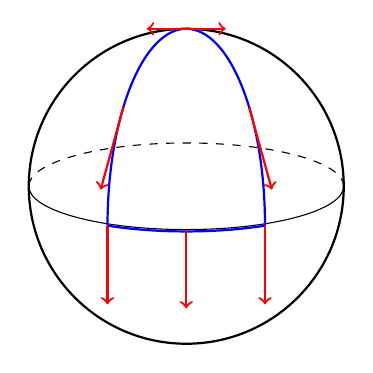
\begin{tikzpicture}
		%\draw[help lines] (-2,-2) grid (2,2);
		
		%SFERA
		\draw[thick] (0,0)circle (2);
		\draw (-2,0) arc (180:360: 2 and 0.55);
		\draw [dashed] (2,0) arc (0:180: 2 and 0.55);
		
		%TRIANGOLO
		\draw[thick, blue] (0,2) arc (90:180: 1 and 2.5);
		\draw[thick,blue] (-1,-.5) arc (240:300: 2 and 0.55);
		\draw[thick, blue] (1,-.5) arc (0:90: 1 and 2.5);
		
		%CAMPO VETTORIALE
		\draw[thick, red, ->] (0,2) to (-0.5, 2);
		\draw[thick, red, ->] (-0.8,1) to (-1.087,-0.042);
		\draw[thick, red, ->] (-1, -.5) to (-1,-1.5);
		\draw[thick, red, ->] (0,-.55) to (0,-1.55);
		\draw[thick, red, ->] (1, -.5) to (1,-1.5);
		\draw[thick, red, ->] (0,2) to (0.5, 2);
		\draw[thick, red, ->] (0.8,1) to (1.087,-0.042);
	\end{tikzpicture}
	
	\caption{In blu il triangolo geodetico \(\gamma\), con \(\gamma(0)=\gamma(1) = (0,0,1)\) e orientata in senso antiorario. In rosso il campo \(V\), ottenuto trasportando parallelemanete \(V_0 = \dot \gamma(0)\).}
	
	\label{fig: trasporto parallelo sulla sfera}
\end{figure}